\originalchapter{8.04 作业6：能态干涉与数值打靶}
来源为Spring 2016 Assignment 6, Barton Zwiebach. 第1、3--6题有实际完整题面, 以下中文转述, 解答均为\textbf{AI独立解答}. 部分原页眉沿用Fall 2015, 与网页托管学期分别保留. 第2题仅Griffiths 2.45、p.87引用, 不补造; 一维非简并的独立证明见正文.
\originalsection{第1题：无限井的两个能态}
\begin{exercise}
长度$a$无限井初态$\psi(0)=u_2/\sqrt3+\sqrt{2/3}u_3$. (a)是否为能态, 求时间态. (b)测得$E_*,4E_*,9E_*$的概率,$E_*=\pi^2\hbar^2/(2ma^2)$. (c)(d)求$\langle x\rangle(t),\langle p\rangle(t)$.
\end{exercise}
\begin{solution}
$u_n=\sqrt{2/a}\sin(n\pi x/a)$, 两项异能故非能量本征态. $\psi(t)=u_2\e^{-4\ii E_*t/\hbar}/\sqrt3+\sqrt{2/3}u_3\e^{-9\ii E_*t/\hbar}$. 三读数概率为$0,1/3,2/3$, 时间相位不改能量分布.

对角位置均为$a/2$, 积分给
\[
\int_0^a\frac{2x}{a}\sin\frac{2\pi x}{a}\sin\frac{3\pi x}{a}\dd x=-\frac{48a}{25\pi^2}.
\]
 因此位置均值和动量均值分别为
\begin{align*}
\langle x\rangle&=\frac a2-\frac{32\sqrt2a}{25\pi^2}\cos\frac{5E_*t}{\hbar},\\
\langle p\rangle&=\frac{16\sqrt2\hbar}{5a}\sin\frac{5E_*t}{\hbar}.
\end{align*}
动量可独立积分, 亦由$\mathrm d\langle x\rangle/\mathrm dt=\langle p\rangle/m$核验. 初态实使$t=0$动量0, 这是符号检验; 不能仅加权两个能态各自位置均值而漏交叉干涉.
\end{solution}
\originalsection{第3题：矩形井简并}
\begin{exercise}
二维矩形硬井边长$L_x,L_y$, 求归一本征函数与能谱. 正方形有哪些简并? 若$(L_x/L_y)^2$无理, 证明无简并.
\end{exercise}
\begin{solution}
分离变量给$u_{nm}=2\sin(n\pi x/L_x)\sin(m\pi y/L_y)/\sqrt{L_xL_y}$, $n,m$正整数; 能谱为
\[
E_{nm}=\frac{\pi^2\hbar^2}{2m_{\rm particle}}\left(\frac{n^2}{L_x^2}+\frac{m^2}{L_y^2}\right).
\]
 此处第二下标$m$与质量区别以$ m_{\rm particle}$记. 正方形$n\ne m$交换对给二重简并; 还可能有意外相等平方和, 例如$1^2+7^2=5^2+5^2=7^2+1^2=50$, 为三重. 若两对等能, 则$n^2-n'^2=-(L_x/L_y)^2(m^2-m'^2)$, 无理系数乘非零整数不可能等整数, 故先$m=m'$, 再$n=n'$. 不能只消除交换简并而忽略其他平方和关系.
\end{solution}
\originalsection{第4题：半井阶势的低能谱}
\begin{exercise}
硬墙在$x=0,2a$, $0<x<a$势0、$a<x<2a$势$V_0$. 对$0<E<V_0$求量子化方程, $z_0^2=2ma^2V_0/\hbar^2$. $z_0=2\pi$求两低能态至四位.
\end{exercise}
\begin{solution}
左段$A\sin kx$,$k=\sqrt{2mE}/\hbar$, 右段$B\sinh[\kappa(2a-x)]$,$\kappa=\sqrt{2m(V_0-E)}/\hbar$. 在$a$函数和导数连续, 消系数得$\eta\cot\eta=-\xi\coth\xi$, $\eta=ka,\xi=\kappa a$, $\eta^2+\xi^2=z_0^2$. 右侧负使左根分别在$(\pi/2,\pi)$与$(3\pi/2,2\pi)$, 没有第三个低于阶势的根. 用不含cot极点的行列式$\sin\eta\cosh\xi+\eta\cos\eta\sinh\xi/\xi=0$求根, 得$E_1/V_0=0.184358065713$, $E_2/V_0=0.707470235821$, 四位小数为0.1844、0.7075.
\end{solution}
\originalsection{第5题：打靶、节点与振幅}
\begin{exercise}
先熟悉四次势$-\psi''/2+(u^4-e)\psi=0$, 偶初值$(1,0)$且试值$e=0.65$, 求基态. 再对前题令$x=au,e=E/V_0$, 用打靶恢复前两能级及第3、4级. 构造八内部节点的第八激发态, 求能量与两侧包络幅度比, 比较局部de Broglie预测.
\end{exercise}
\begin{solution}
四次势初值偶性固定导数0, $e$稍离正确值就混入禁止区增长支. 向内打靶与边值法交叉得到$e_g=0.667986259156$, 高于试值0.65. 远处有限墙不能看作精确无穷边界, 将截断从3.5延到6得到同一前12位作为数值收敛证据.

阶井无量纲方程$-\psi''/z_0^2+f(u)\psi=e\psi$, $f=0$于$(0,1)$、1于$(1,2)$, 初值$\psi(0)=0,\psi'(0)=1$, 求$\psi(2)=0$. $e>1$右段换为$A_R\sin[q(2-u)]$,$q=z_0\sqrt{e-1}$, 左段$A_L\sin\eta u$,$\eta=z_0\sqrt e$. 行列式$\sin\eta\cos q+\eta\cos\eta\sin q/q=0$在$q=0$连续取极限. 前四能量比为0.184358065713、0.707470235821、1.206516570024、1.562500000000. 第4根还有解析校验$\eta=5\pi/2,q=3\pi/2$, 接口两侧导数都0.

沿全部低能根排序, 第9态（第八激发）$e_9=5.557413654033$, 左右各4节点, 硬墙端点不计内部节点. 连续给$|A_L/A_R|=|\sin q/\sin\eta|=0.959735973069$. 慢变近似振幅$\propto\sqrt\lambda$给$\sqrt{q/\eta}=0.951615333682$, 相差约0.85\%. 台阶并不慢变, 此规律仅近似; 精确幅度取接口接续, 不能把采样图当证明.
\begin{center}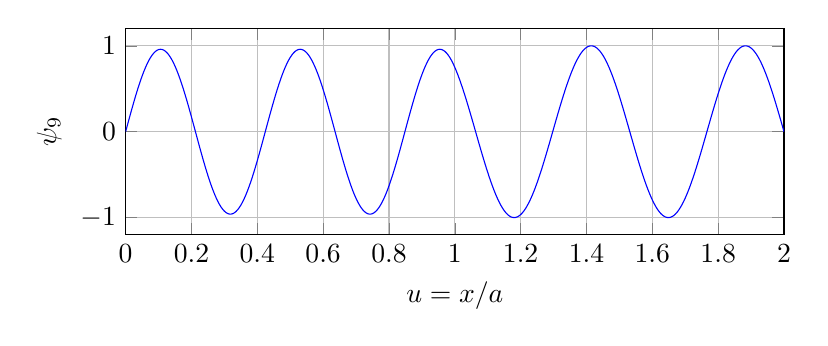
\begin{tikzpicture}
\begin{axis}[width=.82\textwidth,height=4.2cm,xlabel={$u=x/a$},ylabel={$\psi_9$},grid=major,legend style={font=\small},xmin=0,xmax=2]
\addplot+[mark=none] coordinates{(0,0) (0.005,0.0710135006) (0.01,0.141637674) (0.015,0.211485327) (0.02,0.280173524) (0.025,0.347325687) (0.03,0.412573657) (0.035,0.475559716) (0.04,0.535938548) (0.045,0.593379128) (0.05,0.647566542) (0.055,0.69820371) (0.06,0.745013019) (0.065,0.787737837) (0.07,0.82614393) (0.075,0.860020737) (0.08,0.889182531) (0.085,0.913469435) (0.09,0.932748296) (0.095,0.946913421) (0.1,0.955887148) (0.105,0.959620281) (0.11,0.958092352) (0.115,0.951311739) (0.12,0.939315615) (0.125,0.92216975) (0.13,0.899968143) (0.135,0.872832513) (0.14,0.840911632) (0.145,0.804380502) (0.15,0.763439403) (0.155,0.718312794) (0.16,0.669248076) (0.165,0.616514246) (0.17,0.560400413) (0.175,0.501214218) (0.18,0.439280146) (0.185,0.374937746) (0.19,0.308539772) (0.195,0.240450247) (0.2,0.171042468) (0.205,0.100696958) (0.21,0.0297993839) (0.215,-0.0412615639) (0.22,-0.112096298) (0.225,-0.18231647) (0.23,-0.251537103) (0.235,-0.319378699) (0.24,-0.38546932) (0.245,-0.449446629) (0.25,-0.510959872) (0.255,-0.569671809) (0.26,-0.625260553) (0.265,-0.677421344) (0.27,-0.725868212) (0.275,-0.770335551) (0.28,-0.81057957) (0.285,-0.846379635) (0.29,-0.877539474) (0.295,-0.903888254) (0.3,-0.925281521) (0.305,-0.941601986) (0.31,-0.952760175) (0.315,-0.958694912) (0.32,-0.95937366) (0.325,-0.9547927) (0.33,-0.944977145) (0.335,-0.929980809) (0.34,-0.909885908) (0.345,-0.884802611) (0.35,-0.854868436) (0.355,-0.820247496) (0.36,-0.781129597) (0.365,-0.737729202) (0.37,-0.69028425) (0.375,-0.639054855) (0.38,-0.58432188) (0.385,-0.526385395) (0.39,-0.465563033) (0.395,-0.402188249) (0.4,-0.336608492) (0.405,-0.269183299) (0.41,-0.200282324) (0.415,-0.130283313) (0.42,-0.059570032) (0.425,0.0114698384) (0.43,0.0824468262) (0.435,0.152971804) (0.44,0.222658123) (0.445,0.291123732) (0.45,0.357993273) (0.455,0.422900136) (0.46,0.485488474) (0.465,0.545415151) (0.47,0.602351622) (0.475,0.655985735) (0.48,0.706023445) (0.485,0.752190424) (0.49,0.794233563) (0.495,0.831922363) (0.5,0.865050198) (0.505,0.893435447) (0.51,0.916922489) (0.515,0.935382558) (0.52,0.948714447) (0.525,0.956845065) (0.53,0.959729837) (0.535,0.957352947) (0.54,0.949727425) (0.545,0.93689508) (0.55,0.918926262) (0.555,0.895919486) (0.56,0.868000884) (0.565,0.835323519) (0.57,0.798066542) (0.575,0.756434212) (0.58,0.710654777) (0.585,0.660979218) (0.59,0.607679881) (0.595,0.551048974) (0.6,0.491396974) (0.605,0.429050919) (0.61,0.364352618) (0.615,0.297656775) (0.62,0.229329046) (0.625,0.159744035) (0.63,0.0892832363) (0.635,0.0183329475) (0.64,-0.0527178505) (0.645,-0.123479626) (0.65,-0.193564432) (0.655,-0.262588032) (0.66,-0.330172009) (0.665,-0.395945837) (0.67,-0.459548916) (0.675,-0.520632545) (0.68,-0.578861837) (0.685,-0.633917553) (0.69,-0.685497854) (0.695,-0.733319953) (0.7,-0.777121669) (0.705,-0.816662862) (0.71,-0.851726748) (0.715,-0.882121093) (0.72,-0.907679262) (0.725,-0.928261132) (0.73,-0.943753866) (0.735,-0.954072525) (0.74,-0.959160538) (0.745,-0.95899001) (0.75,-0.953561876) (0.755,-0.942905896) (0.76,-0.927080489) (0.765,-0.906172419) (0.77,-0.880296312) (0.775,-0.849594033) (0.78,-0.814233905) (0.785,-0.774409787) (0.79,-0.730340014) (0.795,-0.682266194) (0.8,-0.630451891) (0.805,-0.575181172) (0.81,-0.516757057) (0.815,-0.455499852) (0.82,-0.391745396) (0.825,-0.325843218) (0.83,-0.258154625) (0.835,-0.189050714) (0.84,-0.118910344) (0.845,-0.0481180549) (0.85,0.0229380386) (0.855,0.0938683757) (0.86,0.164284085) (0.865,0.233799116) (0.87,0.302032358) (0.875,0.368609725) (0.88,0.433166211) (0.885,0.495347889) (0.89,0.554813852) (0.895,0.61123808) (0.9,0.664311232) (0.905,0.713742337) (0.91,0.759260391) (0.915,0.800615846) (0.92,0.837581971) (0.925,0.869956103) (0.93,0.897560752) (0.935,0.920244577) (0.94,0.937883216) (0.945,0.950379966) (0.95,0.957666313) (0.955,0.959702312) (0.96,0.9564768) (0.965,0.94800746) (0.97,0.934340725) (0.975,0.915551523) (0.98,0.891742863) (0.985,0.863045277) (0.99,0.829616095) (0.995,0.791638592) (1,0.749320978) (1.005,0.703257421) (1.01,0.654031807) (1.015,0.601865469) (1.02,0.546992963) (1.025,0.489661011) (1.03,0.430127396) (1.035,0.368659799) (1.04,0.305534596) (1.045,0.241035617) (1.05,0.17545287) (1.055,0.109081234) (1.06,0.0422191358) (1.065,-0.0248327924) (1.07,-0.0917730648) (1.075,-0.158300698) (1.08,-0.224116563) (1.085,-0.288924733) (1.09,-0.352433811) (1.095,-0.414358239) (1.1,-0.474419589) (1.105,-0.532347804) (1.11,-0.587882424) (1.115,-0.640773747) (1.12,-0.690783959) (1.125,-0.737688198) (1.13,-0.781275568) (1.135,-0.821350088) (1.14,-0.857731571) (1.145,-0.890256434) (1.15,-0.918778436) (1.155,-0.943169333) (1.16,-0.963319457) (1.165,-0.979138206) (1.17,-0.990554455) (1.175,-0.997516873) (1.18,-0.999994155) (1.185,-0.997975161) (1.19,-0.991468971) (1.195,-0.980504837) (1.2,-0.965132058) (1.205,-0.945419755) (1.21,-0.92145656) (1.215,-0.893350218) (1.22,-0.861227105) (1.225,-0.825231655) (1.23,-0.785525715) (1.235,-0.742287815) (1.24,-0.695712365) (1.245,-0.646008783) (1.25,-0.593400551) (1.255,-0.538124211) (1.26,-0.480428303) (1.265,-0.420572244) (1.27,-0.358825166) (1.275,-0.295464701) (1.28,-0.230775739) (1.285,-0.165049139) (1.29,-0.0985804283) (1.295,-0.0316684704) (1.3,0.0353858784) (1.305,0.102281122) (1.31,0.168716478) (1.315,0.234393235) (1.32,0.299016088) (1.325,0.362294476) (1.33,0.423943878) (1.335,0.483687101) (1.34,0.541255521) (1.345,0.596390293) (1.35,0.648843515) (1.355,0.698379341) (1.36,0.744775043) (1.365,0.787822012) (1.37,0.827326695) (1.375,0.863111469) (1.38,0.895015434) (1.385,0.922895139) (1.39,0.94662523) (1.395,0.966099009) (1.4,0.981228916) (1.405,0.991946922) (1.41,0.998204835) (1.415,0.99997452) (1.42,0.997248017) (1.425,0.990037587) (1.43,0.978375649) (1.435,0.96231464) (1.44,0.941926775) (1.445,0.917303723) (1.45,0.888556197) (1.455,0.855813454) (1.46,0.819222717) (1.465,0.778948507) (1.47,0.735171911) (1.475,0.68808976) (1.48,0.63791375) (1.485,0.584869487) (1.49,0.529195476) (1.495,0.471142042) (1.5,0.410970211) (1.505,0.348950535) (1.51,0.285361872) (1.515,0.220490136) (1.52,0.15462701) (1.525,0.0880686338) (1.53,0.021114275) (1.535,-0.0459350201) (1.54,-0.112777777) (1.545,-0.179113452) (1.55,-0.244643778) (1.555,-0.309074113) (1.56,-0.372114756) (1.565,-0.43348226) (1.57,-0.492900698) (1.575,-0.550102905) (1.58,-0.604831683) (1.585,-0.656840957) (1.59,-0.705896875) (1.595,-0.751778868) (1.6,-0.794280638) (1.605,-0.833211082) (1.61,-0.868395158) (1.615,-0.899674668) (1.62,-0.926908969) (1.625,-0.949975609) (1.63,-0.968770872) (1.635,-0.983210249) (1.64,-0.993228817) (1.645,-0.998781529) (1.65,-0.999843419) (1.655,-0.996409711) (1.66,-0.988495845) (1.665,-0.976137403) (1.67,-0.959389954) (1.675,-0.938328799) (1.68,-0.913048635) (1.685,-0.883663129) (1.69,-0.850304407) (1.695,-0.813122461) (1.7,-0.772284471) (1.705,-0.727974058) (1.71,-0.680390453) (1.715,-0.629747609) (1.72,-0.576273229) (1.725,-0.520207752) (1.73,-0.461803263) (1.735,-0.401322368) (1.74,-0.339037007) (1.745,-0.275227233) (1.75,-0.210179955) (1.755,-0.144187644) (1.76,-0.0775470225) (1.765,-0.0105577259) (1.77,0.0564790414) (1.775,0.123261862) (1.78,0.18949046) (1.785,0.254867052) (1.79,0.319097685) (1.795,0.381893558) (1.8,0.442972323) (1.805,0.502059351) (1.81,0.558888969) (1.815,0.613205654) (1.82,0.664765181) (1.825,0.713335724) (1.83,0.758698894) (1.835,0.800650726) (1.84,0.839002591) (1.845,0.873582048) (1.85,0.904233616) (1.855,0.930819478) (1.86,0.953220095) (1.865,0.971334747) (1.87,0.985081986) (1.875,0.994399999) (1.88,0.99924689) (1.885,0.999600867) (1.89,0.995460336) (1.895,0.986843916) (1.9,0.973790349) (1.905,0.956358327) (1.91,0.934626229) (1.915,0.908691771) (1.92,0.878671561) (1.925,0.844700578) (1.93,0.806931567) (1.935,0.765534349) (1.94,0.720695058) (1.945,0.672615305) (1.95,0.621511271) (1.955,0.567612735) (1.96,0.511162041) (1.965,0.452413008) (1.97,0.39162979) (1.975,0.329085687) (1.98,0.265061916) (1.985,0.199846346) (1.99,0.133732207) (1.995,0.0670167671) (2,0)};
\end{axis}\end{tikzpicture}\end{center}
\begin{center}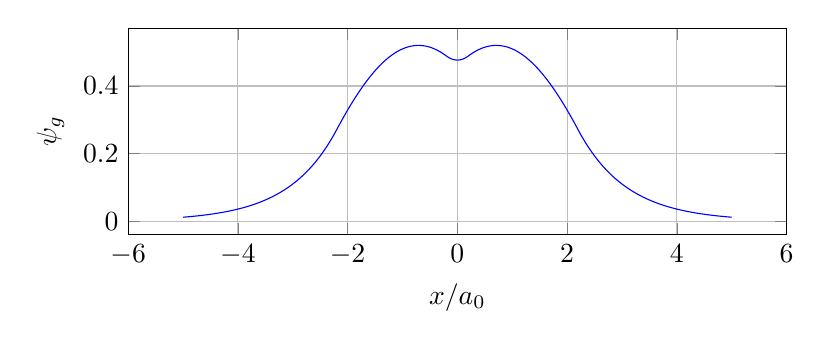
\begin{tikzpicture}
\begin{axis}[width=.82\textwidth,height=4.2cm,xlabel={$x/a_0$},ylabel={$\psi_g$},grid=major,legend style={font=\small},]
\addplot+[mark=none] coordinates{(-5,0.0115418908) (-4.975,0.0118715894) (-4.95,0.012210706) (-4.925,0.0125595096) (-4.9,0.0129182769) (-4.875,0.0132872925) (-4.85,0.0136668492) (-4.825,0.014057248) (-4.8,0.0144587988) (-4.775,0.01487182) (-4.75,0.0152966393) (-4.725,0.0157335938) (-4.7,0.01618303) (-4.675,0.0166453046) (-4.65,0.0171207842) (-4.625,0.0176098461) (-4.6,0.0181128782) (-4.575,0.0186302796) (-4.55,0.0191624608) (-4.525,0.019709844) (-4.5,0.0202728633) (-4.475,0.0208519656) (-4.45,0.0214476101) (-4.425,0.0220602694) (-4.4,0.0226904296) (-4.375,0.0233385906) (-4.35,0.0240052665) (-4.325,0.0246909863) (-4.3,0.0253962939) (-4.275,0.026121749) (-4.25,0.0268679269) (-4.225,0.0276354197) (-4.2,0.0284248362) (-4.175,0.0292368027) (-4.15,0.0300719634) (-4.125,0.0309309807) (-4.1,0.0318145363) (-4.075,0.0327233309) (-4.05,0.0336580856) (-4.025,0.0346195419) (-4,0.0356084626) (-3.975,0.0366256322) (-3.95,0.0376718577) (-3.925,0.0387479689) (-3.9,0.0398548198) (-3.875,0.0409932882) (-3.85,0.0421642775) (-3.825,0.0433687165) (-3.8,0.0446075608) (-3.775,0.0458817931) (-3.75,0.0471924244) (-3.725,0.0485404944) (-3.7,0.0499270725) (-3.675,0.0513532588) (-3.65,0.0528201846) (-3.625,0.0543290138) (-3.6,0.0558809432) (-3.575,0.0574772041) (-3.55,0.0591190629) (-3.525,0.0608078219) (-3.5,0.062544821) (-3.475,0.0643314382) (-3.45,0.0661690908) (-3.425,0.0680592367) (-3.4,0.0700033753) (-3.375,0.072003049) (-3.35,0.0740598441) (-3.325,0.0761753924) (-3.3,0.0783513722) (-3.275,0.0805895096) (-3.25,0.0828915804) (-3.225,0.0852594106) (-3.2,0.0876948789) (-3.175,0.0901999173) (-3.15,0.0927765131) (-3.125,0.0954267103) (-3.1,0.0981526115) (-3.075,0.100956379) (-3.05,0.103840237) (-3.025,0.106806474) (-3,0.109857443) (-2.975,0.112995563) (-2.95,0.116223326) (-2.925,0.11954329) (-2.9,0.122958091) (-2.875,0.126470437) (-2.85,0.130083114) (-2.825,0.133798989) (-2.8,0.137621009) (-2.775,0.141552207) (-2.75,0.145595701) (-2.725,0.149754699) (-2.7,0.1540325) (-2.675,0.158432498) (-2.65,0.162958184) (-2.625,0.167613148) (-2.6,0.172401083) (-2.575,0.177325787) (-2.55,0.182391167) (-2.525,0.187601242) (-2.5,0.192960145) (-2.475,0.198472126) (-2.45,0.20414156) (-2.425,0.209972943) (-2.4,0.215970902) (-2.375,0.222140195) (-2.35,0.228485716) (-2.325,0.2350125) (-2.3,0.241725723) (-2.275,0.248630713) (-2.25,0.255732946) (-2.225,0.263038057) (-2.2,0.270551842) (-2.175,0.278131743) (-2.15,0.285629777) (-2.125,0.293043736) (-2.1,0.300371437) (-2.075,0.307610723) (-2.05,0.314759465) (-2.025,0.321815556) (-2,0.328776922) (-1.975,0.335641511) (-1.95,0.342407305) (-1.925,0.349072311) (-1.9,0.355634567) (-1.875,0.362092142) (-1.85,0.368443136) (-1.825,0.374685678) (-1.8,0.380817931) (-1.775,0.38683809) (-1.75,0.392744384) (-1.725,0.398535073) (-1.7,0.404208453) (-1.675,0.409762854) (-1.65,0.415196642) (-1.625,0.420508216) (-1.6,0.425696014) (-1.575,0.430758508) (-1.55,0.435694208) (-1.525,0.440501661) (-1.5,0.445179453) (-1.475,0.449726206) (-1.45,0.454140582) (-1.425,0.458421281) (-1.4,0.462567044) (-1.375,0.466576651) (-1.35,0.47044892) (-1.325,0.474182713) (-1.3,0.477776929) (-1.275,0.481230513) (-1.25,0.484542445) (-1.225,0.487711753) (-1.2,0.490737503) (-1.175,0.493618803) (-1.15,0.496354808) (-1.125,0.498944709) (-1.1,0.501387747) (-1.075,0.503683201) (-1.05,0.505830395) (-1.025,0.507828698) (-1,0.509677522) (-0.975,0.511376322) (-0.95,0.512924598) (-0.925,0.514321895) (-0.9,0.515567801) (-0.875,0.51666195) (-0.85,0.517604019) (-0.825,0.518393731) (-0.8,0.519030854) (-0.775,0.5195152) (-0.75,0.519846626) (-0.725,0.520025036) (-0.7,0.520050376) (-0.675,0.519922639) (-0.65,0.519641863) (-0.625,0.51920813) (-0.6,0.518621568) (-0.575,0.517882349) (-0.55,0.516990692) (-0.525,0.515946859) (-0.5,0.514751156) (-0.475,0.513403936) (-0.45,0.511905596) (-0.425,0.510256576) (-0.4,0.508457362) (-0.375,0.506508484) (-0.35,0.504410515) (-0.325,0.502164072) (-0.3,0.499769817) (-0.275,0.497228455) (-0.25,0.494540733) (-0.225,0.491707444) (-0.2,0.48872942) (-0.175,0.485872773) (-0.15,0.48340158) (-0.125,0.481313878) (-0.1,0.479608013) (-0.075,0.47828263) (-0.05,0.477336678) (-0.025,0.476769407) (0,0.476580367) (0.025,0.476769407) (0.05,0.477336678) (0.075,0.47828263) (0.1,0.479608013) (0.125,0.481313878) (0.15,0.48340158) (0.175,0.485872773) (0.2,0.48872942) (0.225,0.491707444) (0.25,0.494540733) (0.275,0.497228455) (0.3,0.499769817) (0.325,0.502164072) (0.35,0.504410515) (0.375,0.506508484) (0.4,0.508457362) (0.425,0.510256576) (0.45,0.511905596) (0.475,0.513403936) (0.5,0.514751156) (0.525,0.515946859) (0.55,0.516990692) (0.575,0.517882349) (0.6,0.518621568) (0.625,0.51920813) (0.65,0.519641863) (0.675,0.519922639) (0.7,0.520050376) (0.725,0.520025036) (0.75,0.519846626) (0.775,0.5195152) (0.8,0.519030854) (0.825,0.518393731) (0.85,0.517604019) (0.875,0.51666195) (0.9,0.515567801) (0.925,0.514321895) (0.95,0.512924598) (0.975,0.511376322) (1,0.509677522) (1.025,0.507828698) (1.05,0.505830395) (1.075,0.503683201) (1.1,0.501387747) (1.125,0.498944709) (1.15,0.496354808) (1.175,0.493618803) (1.2,0.490737503) (1.225,0.487711753) (1.25,0.484542445) (1.275,0.481230513) (1.3,0.477776929) (1.325,0.474182713) (1.35,0.47044892) (1.375,0.466576651) (1.4,0.462567044) (1.425,0.458421281) (1.45,0.454140582) (1.475,0.449726206) (1.5,0.445179453) (1.525,0.440501661) (1.55,0.435694208) (1.575,0.430758508) (1.6,0.425696014) (1.625,0.420508216) (1.65,0.415196642) (1.675,0.409762854) (1.7,0.404208453) (1.725,0.398535073) (1.75,0.392744384) (1.775,0.38683809) (1.8,0.380817931) (1.825,0.374685678) (1.85,0.368443136) (1.875,0.362092142) (1.9,0.355634567) (1.925,0.349072311) (1.95,0.342407305) (1.975,0.335641511) (2,0.328776922) (2.025,0.321815556) (2.05,0.314759465) (2.075,0.307610723) (2.1,0.300371437) (2.125,0.293043736) (2.15,0.285629777) (2.175,0.278131743) (2.2,0.270551842) (2.225,0.263038057) (2.25,0.255732946) (2.275,0.248630713) (2.3,0.241725723) (2.325,0.2350125) (2.35,0.228485716) (2.375,0.222140195) (2.4,0.215970902) (2.425,0.209972943) (2.45,0.20414156) (2.475,0.198472126) (2.5,0.192960145) (2.525,0.187601242) (2.55,0.182391167) (2.575,0.177325787) (2.6,0.172401083) (2.625,0.167613148) (2.65,0.162958184) (2.675,0.158432498) (2.7,0.1540325) (2.725,0.149754699) (2.75,0.145595701) (2.775,0.141552207) (2.8,0.137621009) (2.825,0.133798989) (2.85,0.130083114) (2.875,0.126470437) (2.9,0.122958091) (2.925,0.11954329) (2.95,0.116223326) (2.975,0.112995563) (3,0.109857443) (3.025,0.106806474) (3.05,0.103840237) (3.075,0.100956379) (3.1,0.0981526115) (3.125,0.0954267103) (3.15,0.0927765131) (3.175,0.0901999173) (3.2,0.0876948789) (3.225,0.0852594106) (3.25,0.0828915804) (3.275,0.0805895096) (3.3,0.0783513722) (3.325,0.0761753924) (3.35,0.0740598441) (3.375,0.072003049) (3.4,0.0700033753) (3.425,0.0680592367) (3.45,0.0661690908) (3.475,0.0643314382) (3.5,0.062544821) (3.525,0.0608078219) (3.55,0.0591190629) (3.575,0.0574772041) (3.6,0.0558809432) (3.625,0.0543290138) (3.65,0.0528201846) (3.675,0.0513532588) (3.7,0.0499270725) (3.725,0.0485404944) (3.75,0.0471924244) (3.775,0.0458817931) (3.8,0.0446075608) (3.825,0.0433687165) (3.85,0.0421642775) (3.875,0.0409932882) (3.9,0.0398548198) (3.925,0.0387479689) (3.95,0.0376718577) (3.975,0.0366256322) (4,0.0356084626) (4.025,0.0346195419) (4.05,0.0336580856) (4.075,0.0327233309) (4.1,0.0318145363) (4.125,0.0309309807) (4.15,0.0300719634) (4.175,0.0292368027) (4.2,0.0284248362) (4.225,0.0276354197) (4.25,0.0268679269) (4.275,0.026121749) (4.3,0.0253962939) (4.325,0.0246909863) (4.35,0.0240052665) (4.375,0.0233385906) (4.4,0.0226904296) (4.425,0.0220602694) (4.45,0.0214476101) (4.475,0.0208519656) (4.5,0.0202728633) (4.525,0.019709844) (4.55,0.0191624608) (4.575,0.0186302796) (4.6,0.0181128782) (4.625,0.0176098461) (4.65,0.0171207842) (4.675,0.0166453046) (4.7,0.01618303) (4.725,0.0157335938) (4.75,0.0152966393) (4.775,0.01487182) (4.8,0.0144587988) (4.825,0.014057248) (4.85,0.0136668492) (4.875,0.0132872925) (4.9,0.0129182769) (4.925,0.0125595096) (4.95,0.012210706) (4.975,0.0118715894) (5,0.0115418908)};
\end{axis}\end{tikzpicture}\end{center}

\end{solution}
\originalsection{第6题：H2+方井模型的能量基准}
\begin{exercise}
单氢模型尺度$a_0=\hbar^2/(me^2)$,$|E_H|=13.6$eV, 井深$V_0=1.7402|E_H|$. 两相同宽$2a_0$井分居$\gamma a_0<|x|<(2+\gamma)a_0$, 其余势0,$\gamma=0.2$. (a)打靶求最低电子能并画波函数. (b)加入两质子排斥求离子能量, 与实际分子结合比较.
\end{exercise}
\begin{solution}
令$u=x/a_0$, $\varepsilon=E_e/|E_H|$, 方程$-\psi''+v\psi=\varepsilon\psi$, 井内$v=-1.7402$. 最低态偶, 中央$\psi=\cosh\kappa u$,$\kappa=\sqrt{-\varepsilon}$, 在$u=\gamma$给初值. 井内$q=\sqrt{1.7402+\varepsilon}$传播长度2, 记$y=\cosh\kappa\gamma,y'=\kappa\sinh\kappa\gamma$; 末端$Y=y\cos2q+y'\sin2q/q$, $Y'=-qy\sin2q+y'\cos2q$. 外侧衰减要求$Y'+\kappa Y=0$. 最低无节点根$\varepsilon=-1.269228070616$, $E_e=-17.26150176$eV, 两井内双峰而中央不断开, 曲线见图.

质子在两井中心$\pm(1+\gamma)a_0$, 间距$2.4a_0$, 不是中央空隙$0.4a_0$. 排斥$e^2/[2(1+\gamma)a_0]=|E_H|/(1+\gamma)=11.33333333$eV, 总能$E_{\rm ion}=-5.92816843$eV, 相对于自由两质子与电子的零点. 相对$H+p$解离阈值$-13.6$eV却\textbf{高}7.67183157eV, 所以这个指定玩具模型并不预测对解离稳定, 不能因总能负就宣布成键. 实验比较可由\href{https://webbook.nist.gov/cgi/cbook.cgi?ID=C1333740\&Units=SI\&Mask=20}{NIST氢分子气相离子数据}的解离电离阈值$18.078\pm.003$eV减电离能$15.42593\pm.00005$eV, 独立求H2+至$H+p$的解离能约$2.652\pm.003$eV. 此实验能量差为正而玩具模型给负的结合量$-7.6718$eV, 连稳定性都未复现. 引用单一数据事实, 未打包NIST受版权保护的数据库或表格. 本模型也未对核间距变分或包含核零点运动.
\end{solution}
